\documentclass{article}

\usepackage{amsmath} 
\usepackage{graphicx} 
\usepackage{color}
\usepackage{listings} 
\usepackage{url}
%\definecolor{darkgreen}{rgb}{0,0.5,0}

\lstset{language=Python,
    basicstyle=\ttfamily\bfseries,
    commentstyle=\color{red}\itshape,
  stringstyle=\color{green},
  showstringspaces=false,
  keywordstyle=\color{blue}\bfseries}

\title{A Glimpse at Scipy}
\author{FOSSEE}
\date{June 2010}

\begin{document}
\maketitle

\begin{abstract}
This document shows a glimpse of the features of Scipy that will be
explored during this course.
\end{abstract}

\section{Introduction}

SciPy is open-source software for mathematics, science, and
engineering.

SciPy (pronounced ``Sigh Pie'') is a collection of mathematical
algorithms and convenience functions built on the Numpy extension for
Python. It adds significant power to the interactive Python session by
exposing the user to high-level commands and classes for the
manipulation and visualization of data. With SciPy, an interactive
Python session becomes a data-processing and system-prototyping
environment rivaling sytems such as \emph{Matlab, IDL, Octave, R-Lab,
  and Scilab}. \cite{scipy}

%% \begin{quote}
%%         	In 1998, ... I came across Python and its numerical extension
%%       	(Numeric) while I was looking for ways to analyze large data sets
%%       	... using a high-level language. I quickly fell in love with
%%       	Python programming which is a remarkable statement to make about a
%%       	programming language. If I had not seen others with the same view,
%%       	I might have seriously doubted my sanity.  -- Travis Oliphant, Creator of Numpy    
%% \end{quote}

\subsection{Sub-packages of Scipy}

SciPy is organized into subpackages covering different scientific
computing domains. These are summarized in the \underline{table
  \ref{subpkg}}.

\begin{table}
  \caption{Sub-packages available in Scipy}
  \label{subpkg}
\begin{tabular}{|l|l|}
\hline

\textbf{Subpackage} & \textbf{Description}\\

\hline

\texttt{cluster} & Clustering algorithms\\

\hline

\texttt{constants} & Physical and mathematical constants\\

\hline

\texttt{fftpack} & Fast Fourier Transform routines\\

\hline

\texttt{integrate} & Integration and ordinary differential equation
solvers\\

\hline

\texttt{interpolate} & Interpolation and smoothing splines\\

\hline

\texttt{io} & Input and Output\\

\hline

\texttt{linalg} & Linear algebra\\

\hline

\texttt{maxentropy} & Maximum entropy methods\\

\hline

\texttt{ndimage} & N-dimensional image processing\\

\hline

\texttt{odr} & Orthogonal distance regression\\

\hline

\texttt{optimize} & Optimization and root-finding routines\\

\hline

\texttt{signal} & Signal processing\\

\hline

\texttt{sparse} & Sparse matrices and associated routines\\

\hline

\texttt{spatial} & Spatial data structures and algorithms\\

\hline

\texttt{special} & Special functions\\

\hline

\texttt{stats} & Statistical distributions and functions\\

\hline

\texttt{weave} & C/C++ integration\\

\hline
\end{tabular}
\end{table}

\subsection{Use of Scipy in this course}
Following is a partial list of tasks we shall perform using Scipy, in
this course.

\begin{enumerate}
  \item Plotting \footnote{using \texttt{pylab} - see Appendix
    \ref{mpl}}
  \item Matrix Operations
  \begin{itemize}
    \item Inverse
    \item Determinant
  \end{itemize}
  \item Solving Equations
  \begin{itemize}
    \item System of Linear equations
    \item Polynomials
    \item Non-linear equations
  \end{itemize}
  \item Integration 
  \begin{itemize}
    \item Quadrature
    \item ODEs
  \end{itemize}
\end{enumerate}
\section{A Glimpse of Scipy functions}

This section gives a brief overview of the tasks that are going to be
performed using Scipy, in future classes of this course.

\subsection{Matrix Operations}

Let $\mathbf{A}$ be the matrix 
\(
\begin{bmatrix}
1 &3 &5\\
2 &5 &1\\
2 &3 &8
\end{bmatrix}
\) 

To input $\mathbf{A}$ matrix into python, we do the following in
\texttt{ipython}\footnote{\texttt{ipython} must be started with
  \texttt{-pylab} flag}\\

\begin{lstlisting}
  In []: A = array([[1,3,5],[2,5,1],[2,3,8]])
\end{lstlisting}

\subsubsection{Inverse}

The inverse of a matrix $\mathbf{A}$ is the matrix $\mathbf{B}$ such
that $\mathbf{A}\mathbf{B} = \mathbf{I}$ where $\mathbf{I}$ is the
identity matrix consisting of ones down the main diagonal. Usually
$\mathbf{B}$ is denoted $\mathbf{B} = \mathbf{A}^{-1}$ . In SciPy, the
matrix inverse of matrix $\mathbf{A}$ is obtained using

\lstinline+inv(A)+.
\begin{lstlisting}
  In []: inv(A)
  Out[]: 
  array([[-1.48,  0.36,  0.88],
         [ 0.56,  0.08, -0.36],
         [ 0.16, -0.12,  0.04]])
\end{lstlisting}

\subsubsection{Determinant}

The determinant of a square matrix $\mathbf{A}$ is denoted
$\left|\mathbf{A}\right|$. Suppose $a_{ij}$ are the elements of the
matrix $\mathbf{A}$ and let
$\mathbf{M}_{ij}=\left|\mathbf{A}_{ij}\right|$ be the determinant of
the matrix left by removing the $i^{th}$ row and $j^{th}$ column from
$\mathbf{A}$. Then for any row $i$

    \[ \left|\mathbf{A}\right|=\sum_{j}\left(-1\right)^{i+j}a_{ij}\mathbf{M}_{ij} \]

This is a recursive way to define the determinant where the base case
is defined by accepting that the determinant of a $1\times1$ matrix is
the only matrix element. In SciPy the determinant can be calculated
with $det$ . For example, the determinant of

    \[ \mathbf{A}=\begin{bmatrix} 1 & 3 & 5\\ 2 & 5 & 1\\ 2 & 3 & 8\end{bmatrix}\]

is

    \begin{eqnarray*} 
      |\mathbf{A}| & = & 1\begin{vmatrix} 5 & 1\\ 3 & 8\end{vmatrix}
                        -3\begin{vmatrix} 2 & 1\\ 2 & 8\end{vmatrix}
                        +5\begin{vmatrix}2 & 5\\ 2 & 3\end{vmatrix}\\  
                   & = & 1(5\cdot8-3\cdot1)-3(2\cdot8-2\cdot1)+5(2\cdot3-2\cdot5)=-25
    \end{eqnarray*}

In SciPy, this is computed as shown below

\begin{lstlisting}
  In []: A = array([[1, 3, 5], [2, 5, 1], [2, 3, 8]])
  In []: det(A)
  Out[]: -25.0
\end{lstlisting}

\subsection{Solving Equations}

\subsubsection{Linear Equations}

Solving linear systems of equations is straightforward using the scipy
command \lstinline+solve+. This command expects an input matrix and a
right-hand-side vector. The solution vector is then computed. An
option for entering a symmetrix matrix is offered which can speed up
the processing when applicable.  As an example, suppose it is desired
to solve the following simultaneous equations:

    \begin{eqnarray} x+3y+5z & = & 10\\ 2x+5y+z & = & 8\\ 2x+3y+8z & = & 3\end{eqnarray}

We could find the solution vector using a matrix inverse:

    \[ \left[\begin{array}{c} x\\ y\\ z\end{array}\right]=\left[\begin{array}{ccc} 1 & 3 & 5\\ 2 & 5 & 1\\ 2 & 3 & 8\end{array}\right]^{-1}\left[\begin{array}{c} 10\\ 8\\ 3\end{array}\right]=\frac{1}{25}\left[\begin{array}{c} -232\\ 129\\ 19\end{array}\right]=\left[\begin{array}{c} -9.28\\ 5.16\\ 0.76\end{array}\right] \]

However, it is better to use the solve command which can be faster and
more numerically stable. In this case it however gives the same
answer.

\begin{lstlisting}
  In []: A = array([[1, 3, 5], [2, 5, 1], [2, 3, 8]])
  In []: b = array([[10], [8], [3]])
  In []: dot(inv(A), b)
  Out[]: 
  array([[-9.28],
         [ 5.16],
         [ 0.76]])

  In []: solve(A,b)
  Out[]: 
  array([[-9.28],
         [ 5.16],
         [ 0.76]])
\end{lstlisting}

\subsubsection{Polynomials}

Solving a polynomial is straightforward in scipy using the
\lstinline+roots+ command. It expects the coefficients of the
polynomial in their decreasing order. For example, let's find the
roots of $x^3 - 2x^2 - \frac{1}{2}x + 1$ are $2$, $\sqrt{2}$ and
$-\sqrt{2}$. This is easy to see.

\begin{align*}
x^3 - 2x^2 - \frac{1}{2}x + 1 = 0\\
x^2(x-2) - \frac{1}{2}(x-2) = 0\\
(x-2)(x^2 - \frac{1}{2}) = 0\\
(x-2)(x - \frac{1}{\sqrt{2}})(x + \frac{1}{\sqrt{2}}) = 0
\end{align*}

We do it in scipy as shown below:
\begin{lstlisting}
  In []: coeff = array([1, -2, -2, 4])
  In []: roots(coeff)
\end{lstlisting}

\subsubsection{Non-linear Equations}

To find a root of a set of non-linear equations, the command
\lstinline+fsolve+ is needed. For example, the following example finds
the roots of the single-variable transcendental equation

    \[ x+2\cos\left(x\right)=0,\]

and the set of non-linear equations

    \begin{align} 
      x_{0}\cos\left(x_{1}\right) &= 4,\\ 
      x_{0}x_{1}-x_{1} &= 5
    \end{align}

The results are $x=-1.0299$ and $x_{0}=6.5041,\, x_{1}=0.9084$ .

\begin{lstlisting}
In []: def func(x):
   ...:     return x + 2*cos(x)

In []: def func2(x):
  ...:     out = [x[0]*cos(x[1]) - 4]
  ...:     out.append(x[1]*x[0] - x[1] - 5)
  ...:     return out

In []: from scipy.optimize import fsolve
In []: x0 = fsolve(func, 0.3)
In []: print x0
-1.02986652932

In []: x02 = fsolve(func2, [1, 1])
In []: print x02
[ 6.50409711  0.90841421]
\end{lstlisting}

\subsection{Integration}
% To be done in the lab. 
\subsubsection{Quadrature}

The function \texttt{quad} is provided to integrate a function of one
variable between two points. The points can be $\pm\infty$ ($\pm$
\texttt{inf}) to indicate infinite limits. For example, suppose you
wish to integrate the expression $e^{\sin(x)}$ in the interval
$[0,2\pi]$, i.e. $\int_0^{2\pi}e^{\sin(x)}dx$, it could be computed
using

\begin{lstlisting}
In []: def func(x):
   ...:     return exp(sin(x))

In []: from scipy.integrate import quad
In []: result = quad(func, 0, 2*pi)
In []: print result
(7.9549265210128457, 4.0521874164521979e-10)
\end{lstlisting}

\subsubsection{ODE}

We wish to solve an (a system of) Ordinary Differential Equation. For
this purpose, we shall use \lstinline{odeint}. As an illustration, let
us solve the ODE 

\begin{align} 
  \frac{dy}{dt} = ky(L-y)\\ 
  L = 25000,\,k = 0.00003,\,y(0) = 250 \nonumber 
\end{align}

We solve it in scipy as shown below. 

\begin{lstlisting}
In []: from scipy.integrate import odeint
In []: def f(y, t):
  ...:     k, L = 0.00003, 25000
  ...:     return k*y*(L-y)
  ...:
In []: t = linspace(0, 12, 60)
In []: y0 = 250
In []: y = odeint(f, y0, t)
\end{lstlisting}

Note: To solve a system of ODEs, we need to change the function to
return the right hand side of all the equations and the system and the
pass the required number of initial conditions to the
\lstinline{odeint} function.

\appendix

\section{Plotting using Pylab}\label{mpl}

The following piece of code, produces the plot in Figure \ref{fig:sin}
using \texttt{pylab}\cite{pylab} in \texttt{ipython}\footnote{start
  \texttt{ipython} with \texttt{-pylab} flag}\cite{ipy}

\begin{lstlisting}
In []: x = linspace(0, 2*pi, 50)
In []: plot(x, sin(x))
In []: title('Sine Curve between 0 and $\pi$')
In []: legend(['sin(x)'])
\end{lstlisting}

\begin{figure}[h!]
  \begin{center}
    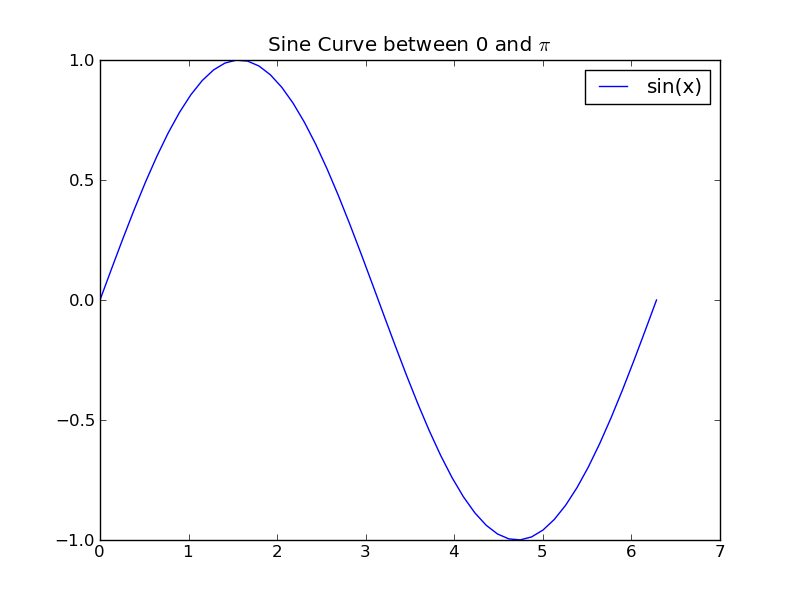
\includegraphics[scale=0.4]{sine}    
  \end{center}
  \caption{Sine curve}
  \label{fig:sin}
\end{figure}



\begin{thebibliography}{9}
  \bibitem{scipy} 
    Eric Jones and Travis Oliphant and Pearu Peterson and others,
    \emph{SciPy: Open source scientific tools for Python}, 2001 -- , 
    \url{http://www.scipy.org/} 

  \bibitem{pylab}
   John D. Hunter, ``Matplotlib: A 2D Graphics Environment,''
   \emph{Computing in Science and Engineering}, vol. 9, no. 3,
   pp. 90-95, May/June 2007, doi:10.1109/MCSE.2007.55 

  \bibitem{ipy}
    Fernando Perez, Brian E. Granger, ``IPython: A System for
    Interactive Scientific Computing,'' \emph{Computing in Science and
    Engineering}, vol.~9, no.~3, pp.~21-29, May/June 2007,
    doi:10.1109/MCSE.2007.53. 

\end{thebibliography}
\end{document}
